\documentclass{article}

\usepackage[a4paper, total={7in, 10in}]{geometry}
\usepackage{tikz-qtree}
\usepackage{enumitem}
\usepackage{titlesec}

\titleformat*{\section}{\Large\bfseries}
\titleformat*{\subsection}{\large\bfseries}
\titleformat*{\subsubsection}{\normalsize\bfseries}
\titleformat*{\paragraph}{\normalsize\bfseries}
\titleformat*{\subparagraph}{\normalsize\bfseries}
\setlength\parindent{0pt}

\renewcommand{\thesubsection}{\thesection.\alph{subsection}}

\begin{document}

\Large\textbf{PROBLEM SET 2: SYNTAX} \\
\normalsize
Alice McKean \\
\today

\section{Tree Drawing}
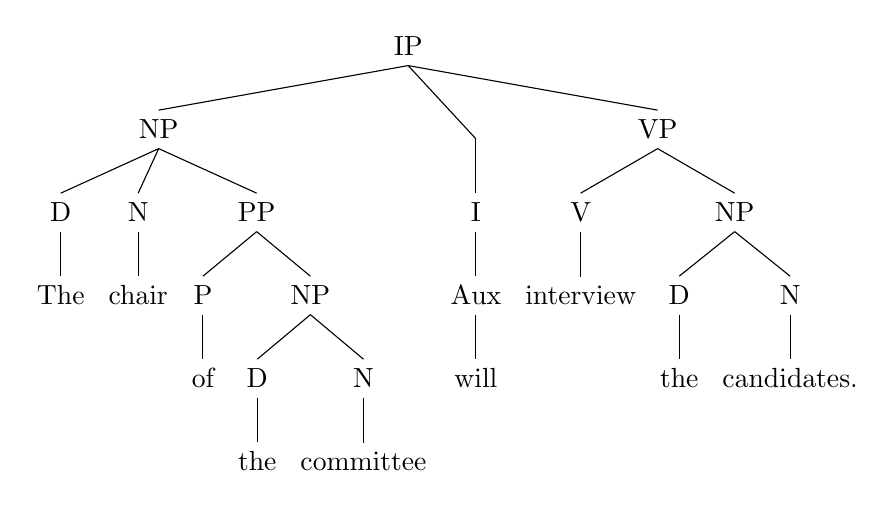
\begin{tikzpicture}
\Tree [.IP [.NP [.D The ]
                [.N chair ]
                [.PP [.P of ]
                    [.NP [.D the ]
                          [.N committee ]
                    ]
                ]
          ]
          [ [.I [.Aux will ] ] ]
          [.VP [.V interview ]
                [.NP [.D the ]
                    [.N candidates. ]
                ]
          ]
      ]
\end{tikzpicture}

\hfill

\begin{tikzpicture}
\Tree [.IP [.NP [.N Drew ] ]
           [.I  [.[Pres] ] ]
           [.VP [.V believes ]
                [.CP [.C that ]
                     [.IP [.NP [.D an ] [.N informant ] ]
                          [.[Past] ]
                          [.VP [.V gave ]
                              [.NP [.NP [.N his ] ]
                                   [.N name ]
                              ]
                              [.PP [.P to ]
                                    [.NP [.D the ]
                                        [.N authorities. ]
                                    ]
                              ]
                          ] 
                     ]
                ]
           ]
      ]
\end{tikzpicture}

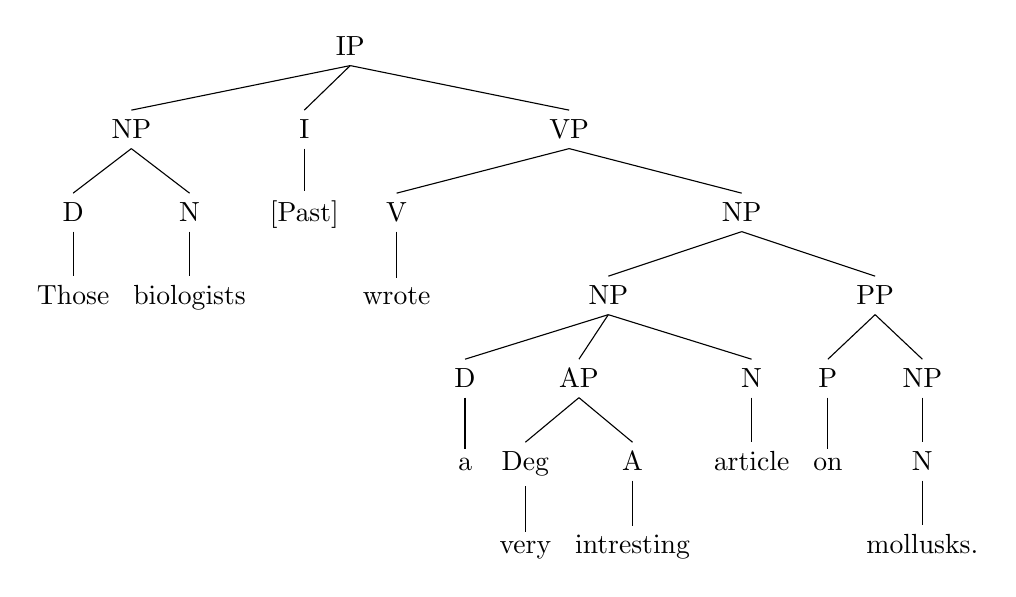
\begin{tikzpicture}
\Tree [.IP [.NP [.D Those ]
                [.N biologists ]
           ]
           [.I [.[Past] ] ]
           [.VP [.V wrote ]
                [.NP [.NP [.D a ]
                          [.AP [.Deg very ]
                               [.A intresting ]
                          ]
                          [.N article ]
                     ]
                     [.PP [.P on ]
                          [.NP [.N mollusks. ] ]
                     ]
                ]
           ]
      ]
\end{tikzpicture}

\section{Structural Ambiguity and Constituency Tests}

\begin{enumerate}[label=(\alph*)]
    \item Paraphrase: `Lucretia used binoculars to spot a wombat.'
    \item Constituency Tests: In this tree `spotted the wombat' is a
      constituent that doesn't appear in B. This claim is supported by the VP
      sentence fragment test as a
      sensible answer to the question, `What did Lucretia do?' is `spotted a
      wombat'. This constituent can also be coordinated with another VP as in
      the following sentence, `Lucretia spotted the wombat and identified the
      cat with the binoculars.' `Lucretia did so with the binoculars' is also a
      grammatical sentence, so this constituent passes the VP did so test.
\end{enumerate}

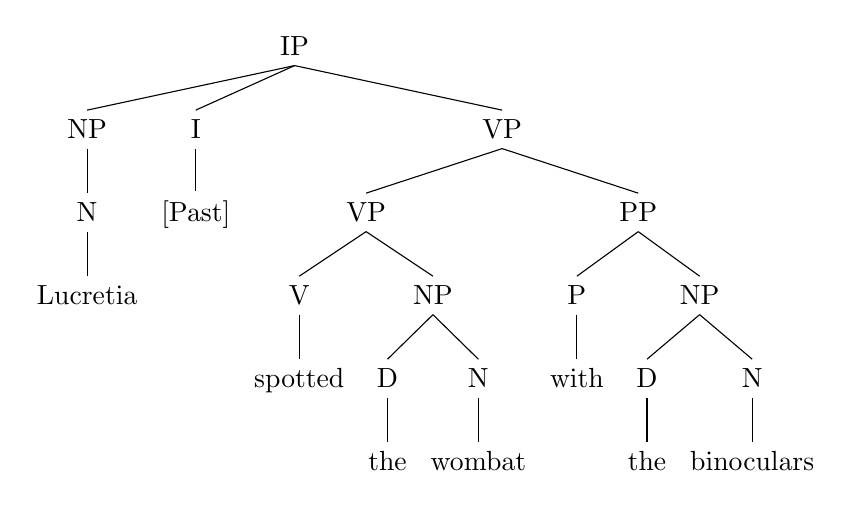
\begin{tikzpicture}
\Tree [.IP [.NP [.N Lucretia ] ]
           [.I  [.[Past] ] ]
           [.VP [.VP [.V spotted ]
                     [.NP [.D the ]
                          [.N wombat ]
                     ]
                ]
                [.PP [.P with ]
                     [.NP [.D the ]
                          [.N binoculars ]
                     ]
                ]
           ]
      ]
\end{tikzpicture}

\begin{enumerate}[label=(\alph*)]
    \item Paraphrase: `A wombat with binoculars was spotted by Lucretia.'
    \item Constituency Tests: In this tree `the wombat with the binoculars' is a
      constituent that doesn't appear in A. This constituent passes the NP
      sentence fragment test because `What did Lucretia spot?' can be answered
      with the sentence fragment `the wombat with the binoculars.' In the
      sentence `Lucretia spotted it'
      the constituent in question was replaced by the pronoun it so the
      constituent passes the NP pronoun replacement test. The following two
      sentences are grammatical `The wombat with the binoculars is what Lucretia
      spotted' and `What Lucretia spotted is the wombat with the binoculars' so
      this constituent can be NP pseudo-clefted. The constituent passes the NP
      coordination test because `Lucretia spotted the wombat with the binoculars
      and the cat' is a grammatical sentence.
\end{enumerate}

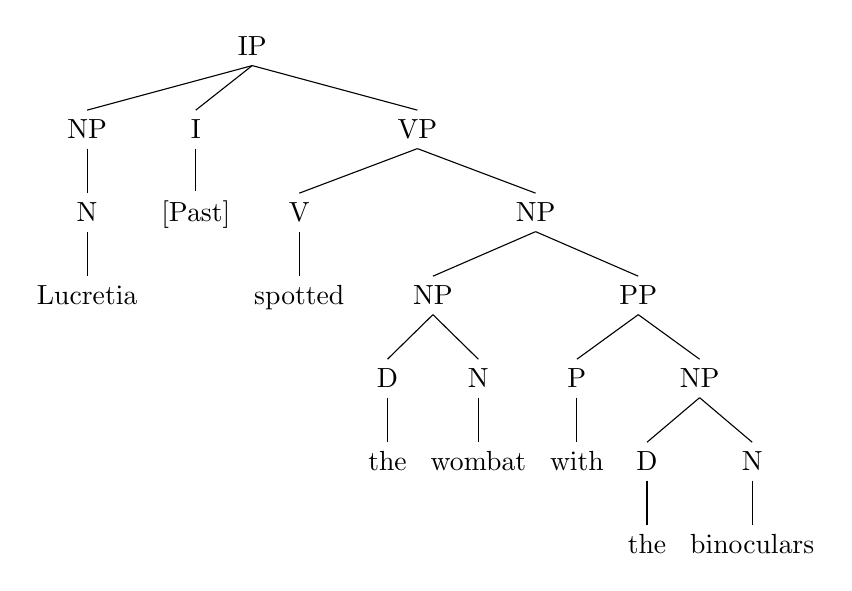
\begin{tikzpicture}
\Tree [.IP [.NP [.N Lucretia ] ]
           [.I  [.[Past] ] ]
           [.VP [.V spotted ]
                [.NP [.NP [.D the ]
                          [.N wombat ]
                     ]
                     [.PP [.P with ]
                          [.NP [.D the ]
                               [.N binoculars ]
                          ]
                     ]
                ]
           ]
      ]
\end{tikzpicture}

\newpage

\section{Acceptability Judgements}
\begin{enumerate}[label=(\theenumi)]
\setcounter{enumi}{4}
\item
  \begin{enumerate}[label=\alph*.]
  \item Grammatical
  \item Pragmatically anomalous as this sentence is fully grammatical but
    implies that your height can change notability in the span of a week.
  \end{enumerate}
\item
  \begin{enumerate}[label=\alph*.]
  \item Grammatical
  \item Ungrammatical an English speaker would not refer to themselves with a
    third person possessive pronoun.
  \item Ungrammatical similar reason as for b with the added benfit of being
    obviously wrong even without indexes.
  \end{enumerate}
\item
  \begin{enumerate}[label=\alph*.]
  \item Stigmatized as plenty of people use `Me and X' but the ``proper''
    alternative is `X and I'.
  \end{enumerate}
\item
  \begin{enumerate}[label=\alph*.]
  \item Grammatical
  \item Grammatical
  \item Ungrammatical as gave back is a Prepositional Verb (Radford 99).
  \item Grammatical
  \item Grammatical
  \item Grammatical
  \end{enumerate}
\end{enumerate}
The people interviewed did surprisingly well and didn't stray far from the
analysis given above. Most of the difference came from 8a as they couldn't see
the indexes because of this they thought the sentence was grammatical. Two of
them commented that the sentence only makes sense if Agnes uses he/him pronouns.
\end{document}